\begin{figure}
\begin{minipage}[ht]{0.45\textwidth}
    \begin{subfloat}[]{
\begin{tikzpicture}[scale=0.45, auto = left,
measure/.style = {very thin,
        {Bar[width=2.2mm]Straight Barb[]}-%
        {Straight Barb[]Bar[width=2.2mm]},
            },
every label/.append style = {font=\footnotesize}]

        \coordinate (LE_R) at ( 0, 0, 0 );
        \coordinate (TE_R) at ( 9.1428, 0, 0 );
        \coordinate (LE_T) at ( 10.609, 16, 0 );
        \coordinate (TE_T) at ( 14.266, 16, 0 );
        \draw[very thick,black] (LE_R) -- (TE_R);
        \draw[very thick,black] (LE_T) -- (TE_T);
        \draw[very thick,black] (LE_T) -- (LE_R);
        \draw[very thick,black] (TE_R) -- (TE_T);
        
        \coordinate (AC_R) at ( 2.28575, 0, 0 );
        \coordinate (AC_T) at ( 11.5233, 16, 0 );
        \draw[very thick,red] (AC_R) -- (AC_T);
        
        \coordinate (Text_Sweep) at ( 4.6, 4.1, 0 );
        \node [rotate=60,anchor=south] at (Text_Sweep) {\textcolor{red}{25\% of chord line}}; 
        
        \coordinate (AC_RT) at ( 2.28575, 16, 0 );
        \draw[very thick,black,dashed] (AC_R) -- (AC_RT);

        \draw [blue,thick,domain=50:90] plot ({2.28575+7*cos(\x)}, {2.28575+7*sin(\x)});
        
        \coordinate (Text_Sweep_Sym) at ( 4.7, 9, 0 );
        \node [rotate=-20,anchor=south] at (Text_Sweep_Sym) {\textcolor{blue}{Sweep Angle $\lambda$}}; 

        \coordinate (H_R) at ( 6.4, 0, 0 );
        \coordinate (H_T) at ( 13.17, 16, 0 );
        \draw[very thick,brown] (H_R) -- (H_T);
        
        \coordinate (Text_Hinge) at ( 11.5, 12, 0 );
        \node [rotate=67,anchor=south] at (Text_Hinge) {\textcolor{brown}{Hinge line at 70\% chord}}; 
        
        \coordinate (TE_TR) at ( 14.266, 0, 0 );
        \draw[measure]  ($(TE_T)!10mm!90:(TE_TR)$) to [sloped,"Model Semi-Span $b$"] ($(TE_TR)!10mm!-90:(TE_T)$);
        
        \draw[measure]  ($(LE_T)!5mm!90:(TE_T)$) to [sloped,"Tip Chord"] ($(TE_T)!5mm!-90:(LE_T)$);

        \coordinate (LE_MAC) at ( 4.547, 6.857, 0 );
        \coordinate (TE_MAC) at ( 11.339, 6.857, 0 );
        \draw[very thick,green] (LE_MAC) -- (TE_MAC);
        \coordinate (Text_MAC) at ( 8, 7.3, 0 );
        \node [] at (Text_MAC) {\textcolor{green}{MAC}}; 
        
        \draw[measure]  ($(LE_R)!9mm!-90:(TE_R)$) to [sloped,"Root Chord"] ($(TE_R)!9mm! 90:(LE_R)$);
        
    \end{tikzpicture}
}
\end{subfloat}
\end{minipage}
\quad
\begin{minipage}[ht]{0.45\textwidth}
\begin{subfloat}[]{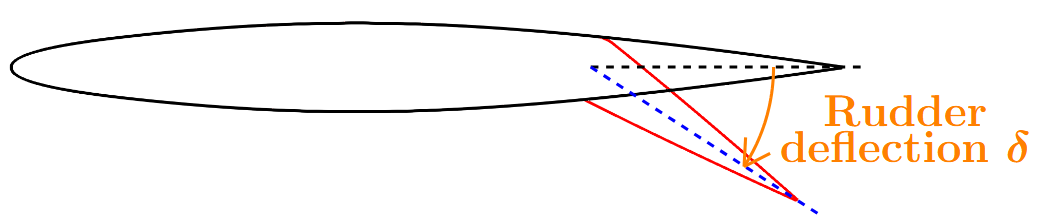
\includegraphics[width=1\textwidth]{FlapDeflection.png}\label{figure:PlanformDefinition:Rudder}}
\end{subfloat}
\begin{subfloat}[]{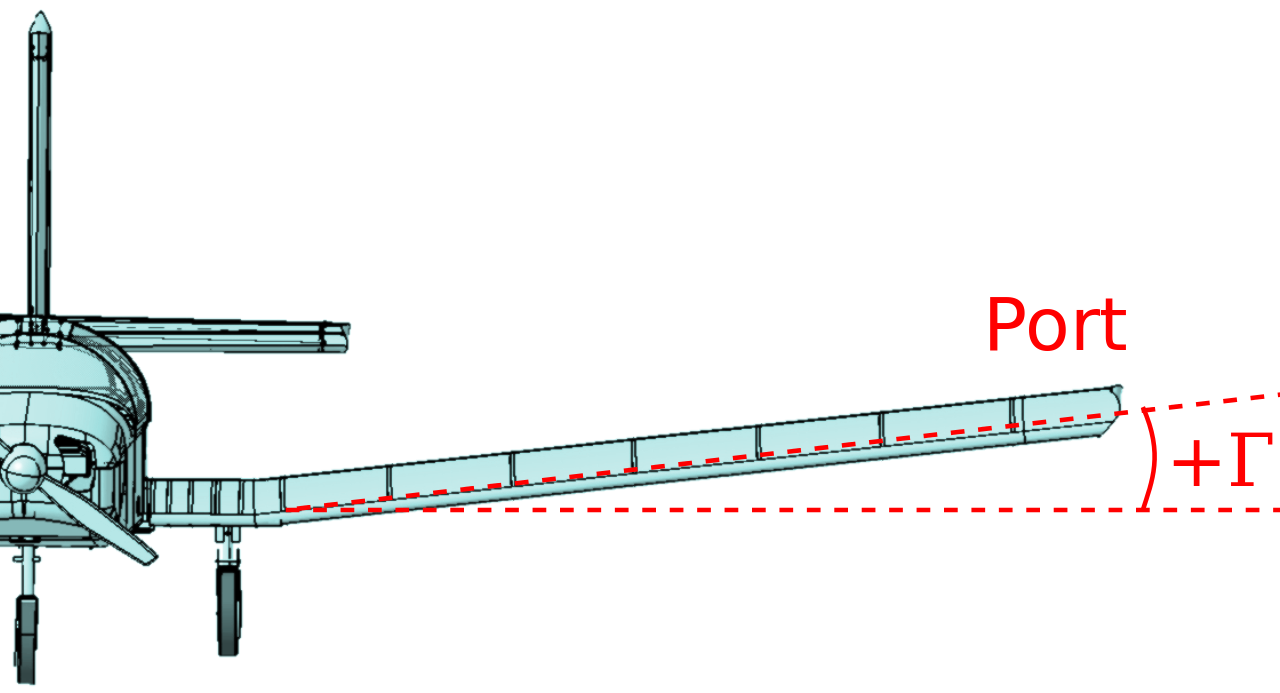
\includegraphics[width=1\textwidth]{Aircraft_dihedral_angle.png}\label{figure:PlanformDefinition:Dihedral}}
\end{subfloat}
\end{minipage}
\caption[Visual definition of geometric parameters]{Planform definition of a trapezoidal lifting surface \cite{rausa2026monnalisa}: \textbf{(a)} in-plane parameters, \textbf{(b)} rudder deflection definition, \textbf{(c)} dihedral angle.}
\label{figure:PlanformDefinition}
\end{figure}
